%!TEX program = xelatex


\documentclass{beamer}
\usepackage{standalone}
\usepackage{import}
\usepackage{csquotes}
\usepackage{appendixnumberbeamer}
\usepackage{csvsimple}
\usepackage{bbding}
\usepackage{amsmath}
\usepackage{amsthm}
\usepackage{amsfonts}
\usepackage{amssymb}

\usetheme{metropolis}
\metroset{block=fill}
\metroset{progressbar=frametitle}
\setbeamertemplate{bibliography item}{}
\setbeamertemplate{caption}{\raggedright\insertcaption\par}

\makeatletter
\def\beamer@framenotesbegin{% at beginning of slide
  \gdef\beamer@noteitems{}%
  \gdef\beamer@notes{{}}% used to be totally empty.
}
\makeatother

\title{Neighborhoods and Segregation: An Information-Theoretic Lens}
\date{\today}
\author{Phil Chodrow}
\institute{MIT Human Mobility and Networks Laboratory \& Operations Research Center}

% \includeonly{tex/slides/intro} will want this later. 

% -------------------------------------------------------------------------------------------------
% -------------------------------------------------------------------------------------------------
% -------------------------------------------------------------------------------------------------

\begin{document}
\maketitle
	%%%%%%%%%%%%%%%%%%%%%%%%%%%%%%%%%%%%%%%%%%%%%%%%%%%%%%%%%%%%%%%%%%%%%%%%%%%%%%%%%%%%%%%%%%%
	\begin{frame}<handout:\included|beamer:\included>\frametitle{Table of contents}
	  \setbeamertemplate{section in toc}[sections numbered]
	  \tableofcontents[hideallsubsections]
	\end{frame}
	%%%%%%%%%%%%%%%%%%%%%%%%%%%%%%%%%%%%%%%%%%%%%%%%%%%%%%%%%%%%%%%%%%%%%%%%%%%%%%%%%%%%%%%%%%%

\section{Introduction}
	%%%%%%%%%%%%%%%%%%%%%%%%%%%%%%%%%%%%%%%%%%%%%%%%%%%%%%%%%%%%%%%%%%%%%%%%%%%%%%%%%%%%%%%%%%
	\begin{frame}\frametitle{Neighborhoods and Diversity}
		Two questions for today: 
		\stepcounter{beamerpauses}
		\begin{enumerate}[<+ ->]
			\item What is \alert<2>{\textbf{urban diversity}}, and how should we measure it? 
			\item What is a \alert<3>{\textbf{neighborhood}}, and how can we distinguish neighborhoods in principled ways?
		\end{enumerate}
		\onslide<4->{
			\begin{block}{Central Claim}
				These two questions are deeply related, and we should approach both using \emph{information theory}.
			\end{block}}
			\note{This is a pretty damn testy note!}
	\end{frame}
	%%%%%%%%%%%%%%%%%%%%%%%%%%%%%%%%%%%%%%%%%%%%%%%%%%%%%%%%%%%%%%%%%%%%%%%%%%%%%%%%%%%%%%%%%%
	%%%%%%%%%%%%%%%%%%%%%%%%%%%%%%%%%%%%%%%%%%%%%%%%%%%%%%%%%%%%%%%%%%%%%%%%%%%%%%%%%%%%%%%%%%%
	\begin{frame}\frametitle{Three Dimensions of Urban Diversity}
	
		\begin{description}[<+ ->]
			\item[\alert<1>{Global diversity}] is the extent to which different groups are equally represented in the city as a whole.  
			\item[\alert<2>{Spatial evenness}] \textit{``or clustering, refers to the extent to which groups are similarly distributed in residential space.''} \cite{Reardon2004}
			\item[\alert<3>{Spatial exposure}] \textit{``refers to the extent that members of one group encounter members of another group (or their own group, in the case of spatial isolation) in their local spatial environments.''} \cite{Reardon2004} 
			
		\end{description}
		
		\onslide<4>{No global diversity $\implies$ perfect evenness $\implies$ maximal exposure.}

	\end{frame}
	%%%%%%%%%%%%%%%%%%%%%%%%%%%%%%%%%%%%%%%%%%%%%%%%%%%%%%%%%%%%%%%%%%%%%%%%%%%%%%%%%%%%%%%%%%%
	%%%%%%%%%%%%%%%%%%%%%%%%%%%%%%%%%%%%%%%%%%%%%%%%%%%%%%%%%%%%%%%%%%%%%%%%%%%%%%%%%%%%%%%%%%%
	\begin{frame}[t]\frametitle{Neighborhoods, Exposure, and the Checkerboard}
	    \textbf{Claim}: Spatial exposure is about the number, scale, and pattern of neighborhoods.
	    \begin{figure}
	    	\centering
	    	\onslide<2->{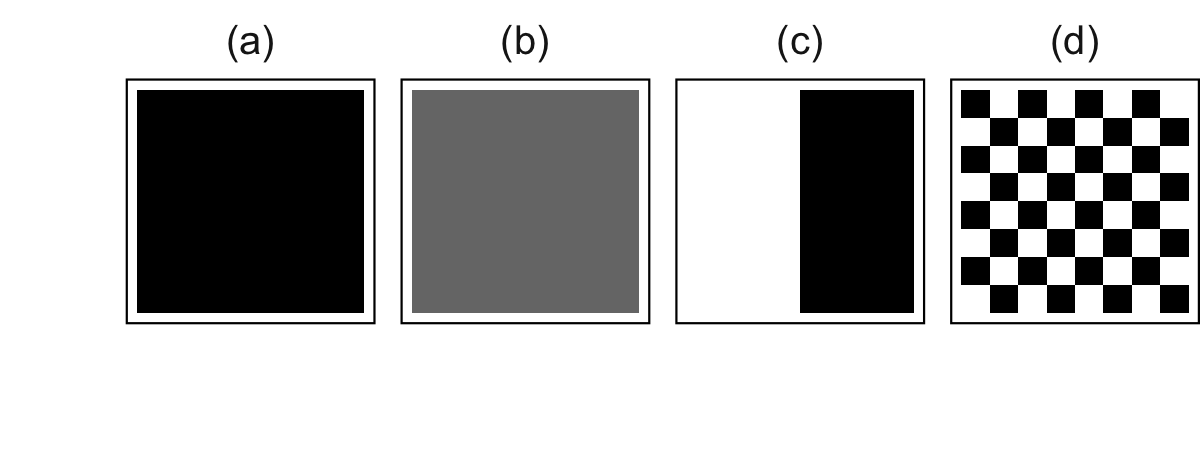
\includegraphics[width=1\textwidth]{figs/checkerboard.png}}

		    \onslide<3->{
			    \begin{tabular}{c | c c c}
			    	City & Exposure & Neighborhoods \\
			    	\hline
			    	(c) & Low & Few, large \\
			    	(d) & High & Many, small
			    \end{tabular}
		    }
	    \end{figure}
	    
	    
	\end{frame}
	%%%%%%%%%%%%%%%%%%%%%%%%%%%%%%%%%%%%%%%%%%%%%%%%%%%%%%%%%%%%%%%%%%%%%%%%%%%%%%%%%%%%%%%%%%%
	%%%%%%%%%%%%%%%%%%%%%%%%%%%%%%%%%%%%%%%%%%%%%%%%%%%%%%%%%%%%%%%%%%%%%%%%%%%%%%%%%%%%%%%%%%%
	\begin{frame}\frametitle{Albuquerque: Low diversity, fairly even, high exposure}
		\begin{figure}
			\includegraphics[width=\textwidth]{external_figs/albuquerque_dot.png}
			\caption{\textit{Image Copyright, 2013, Weldon Cooper Center for Public Service, Rector and Visitors of the University of Virginia (Dustin A. Cable, creator)}}
		\end{figure}
	\end{frame}
	%%%%%%%%%%%%%%%%%%%%%%%%%%%%%%%%%%%%%%%%%%%%%%%%%%%%%%%%%%%%%%%%%%%%%%%%%%%%%%%%%%%%%%%%%%%
	%%%%%%%%%%%%%%%%%%%%%%%%%%%%%%%%%%%%%%%%%%%%%%%%%%%%%%%%%%%%%%%%%%%%%%%%%%%%%%%%%%%%%%%%%%%
	\begin{frame}\frametitle{Detroit: High diversity, highly uneven, low exposure}
		\begin{figure}
			\includegraphics[width=\textwidth]{external_figs/detroit_dot.png}
			\caption{\textit{Image Copyright, 2013, Weldon Cooper Center for Public Service, Rector and Visitors of the University of Virginia (Dustin A. Cable, creator)}}
		\end{figure}
	\end{frame}
	%%%%%%%%%%%%%%%%%%%%%%%%%%%%%%%%%%%%%%%%%%%%%%%%%%%%%%%%%%%%%%%%%%%%%%%%%%%%%%%%%%%%%%%%%%%
	%%%%%%%%%%%%%%%%%%%%%%%%%%%%%%%%%%%%%%%%%%%%%%%%%%%%%%%%%%%%%%%%%%%%%%%%%%%%%%%%%%%%%%%%%%%
	\begin{frame}\frametitle{Philadelphia: High diversity, highly uneven, high exposure}
		\begin{figure}
			\includegraphics[width=\textwidth]{external_figs/philly_dot.png}
			\caption{\textit{Image Copyright, 2013, Weldon Cooper Center for Public Service, Rector and Visitors of the University of Virginia (Dustin A. Cable, creator)}}
		\end{figure}
	\end{frame}
	%%%%%%%%%%%%%%%%%%%%%%%%%%%%%%%%%%%%%%%%%%%%%%%%%%%%%%%%%%%%%%%%%%%%%%%%%%%%%%%%%%%%%%%%%%%
\section{Diversity and Information Theory}
	%%%%%%%%%%%%%%%%%%%%%%%%%%%%%%%%%%%%%%%%%%%%%%%%%%%%%%%%%%%%%%%%%%%%%%%%%%%%%%%%%%%%%%%%%%%
	\begin{frame}\frametitle{Why Information Theory?}
		Information theory quantifies concepts like uncertainty and predictability. Why use it for studying race? 
		\onslide<2->{
			\begin{block}{Core Insight}
				\begin{itemize}
					\item Complex systems allow \textbf{some} prediction...
					\item ...But good prediction is \textbf{hard}.
				\end{itemize}
			\end{block}
		}
		\onslide<3>{
			\textbf{Examples of prediction:}
			\begin{itemize}
				\item If you pick a random person from a city, is it hard to guess their race? ``Yes'' $\implies$ more diverse city. 
				\item Does it help if you tell me where they live? ``Yes'' $\implies$ more uneven city. 
			\end{itemize}
		}
	\end{frame}
	%%%%%%%%%%%%%%%%%%%%%%%%%%%%%%%%%%%%%%%%%%%%%%%%%%%%%%%%%%%%%%%%%%%%%%%%%%%%%%%%%%%%%%%%%%%
	%%%%%%%%%%%%%%%%%%%%%%%%%%%%%%%%%%%%%%%%%%%%%%%%%%%%%%%%%%%%%%%%%%%%%%%%%%%%%%%%%%%%%%%%%%%
	\begin{frame}\frametitle{Entropy as Global Diversity}
		Let $p(X,Y)$ be the joint distribution of location $X$ and race $Y$. The marginal distribution of race alone is $p(Y) = \sum_{x \in \mathcal{X}} p(x,Y)$. 
		\begin{block}{Entropy}
			\begin{equation*}
				H(Y) \triangleq - \mathbb{E}_Y[\log p(Y)] = -\sum_{y \in \mathcal{Y}} p(Y)\log p(Y)
			\end{equation*}
		\end{block}
		\onslide<2->{\begin{align*}
			H(Y) = 0 &\implies \text{ city is monoracial} \\
			H(Y) = \log \left|\mathcal{Y}\right| &\implies \text{ all races are represented equally}
		\end{align*}}
		\onslide<3->{\textbf{Entropy measures global diversity:} more entropy, more diversity.}
	\end{frame}
	%%%%%%%%%%%%%%%%%%%%%%%%%%%%%%%%%%%%%%%%%%%%%%%%%%%%%%%%%%%%%%%%%%%%%%%%%%%%%%%%%%%%%%%%%%%
	%%%%%%%%%%%%%%%%%%%%%%%%%%%%%%%%%%%%%%%%%%%%%%%%%%%%%%%%%%%%%%%%%%%%%%%%%%%%%%%%%%%%%%%%%%%
	\begin{frame}\frametitle{Mutual Information as Evenness}
		The mutual information quantifies the degree of dependence between two random variables.
		\begin{block}{Mutual Information}
			\begin{equation*}
			I(X,Y) \triangleq \sum_{x,y \in \mathcal{X} \times \mathcal{Y}}p(X,Y) \log \frac{p(X,Y)}{p(X)p(Y)}\;.
		\end{equation*}	
		\end{block}
		\onslide<2->{\begin{align*}
			I(X,Y) = 0 &\implies \text{ location and race are independent} \\
			I(X,Y) = \log \left|Y\right| &\implies \text{ location determines race}
		\end{align*}}
		\onslide<3->{\textbf{Mutual information measures evenness:} more information, the more uneven the spatial distribution of demographics.}
	\end{frame}
	%%%%%%%%%%%%%%%%%%%%%%%%%%%%%%%%%%%%%%%%%%%%%%%%%%%%%%%%%%%%%%%%%%%%%%%%%%%%%%%%%%%%%%%%%%%
	%%%%%%%%%%%%%%%%%%%%%%%%%%%%%%%%%%%%%%%%%%%%%%%%%%%%%%%%%%%%%%%%%%%%%%%%%%%%%%%%%%%%%%%%%%%
	\begin{frame}\frametitle{Local Information}
		Let $I_r(x_0)$ be local the mutual information between $X$ and $Y$, restricted to a small area of radius $r$ centered at $x_0$. Think of this as the \textbf{spatial variation of racial trends in a small area.} 
		\onslide<2->{
			\begin{block}{Theorem}
				Under appropriate regularity conditions, for small $r$,
				\begin{equation*}
					\frac{I_r(x_0)}{r^2} \cong \frac{1}{4} \text{trace } J_Y(x_0)\;, \tag{proof on request}
				\end{equation*}
				where $J_Y(x_0)$ is the Fisher information in $Y$ about $x_0$ \nocite{Amari2000}
			\end{block}
		}
		\onslide<3->{
			\alert{Significance}: the local information $I_r(x_0)$ is related to an intrinsic statistical measure $J_Y(x)$ \emph{that is independent of the resolution $r$}.
		} 

	\end{frame}

	%%%%%%%%%%%%%%%%%%%%%%%%%%%%%%%%%%%%%%%%%%%%%%%%%%%%%%%%%%%%%%%%%%%%%%%%%%%%%%%%%%%%%%%%%%%
	%%%%%%%%%%%%%%%%%%%%%%%%%%%%%%%%%%%%%%%%%%%%%%%%%%%%%%%%%%%%%%%%%%%%%%%%%%%%%%%%%%%%%%%%%%%
	\begin{frame}\frametitle{Mean Local Information Measures Spatial Exposure}
		We're interested in the average value of local information: 

		\onslide<2->{
			\begin{block}{Mean Local Information}
				\begin{equation*}
					J(X,Y) \triangleq \mathbb{E}_X[\text{trace } J_Y(X)]\;.
				\end{equation*}
			\end{block}
		}
		\onslide<3->{
			\begin{align*}
				J(X,Y) = 0 &\implies \text{No neighborhoods, low exposure} \\
				J(X,Y) \text{ large} &\implies \text{Lots of neighborhoods, high exposure}
			\end{align*}
		}
		\onslide<4->{
			This is one way of ``spatializing'' the mutual information $I(X,Y)$; for another see \cite{Roberto2015a,Roberto2015}. 
		}
	\end{frame}
	%%%%%%%%%%%%%%%%%%%%%%%%%%%%%%%%%%%%%%%%%%%%%%%%%%%%%%%%%%%%%%%%%%%%%%%%%%%%%%%%%%%%%%%%%%%
	%%%%%%%%%%%%%%%%%%%%%%%%%%%%%%%%%%%%%%%%%%%%%%%%%%%%%%%%%%%%%%%%%%%%%%%%%%%%%%%%%%%%%%%%%%%
	\begin{frame}\frametitle{Back to the checkerboard}
		\begin{figure}
	    	\centering
	    	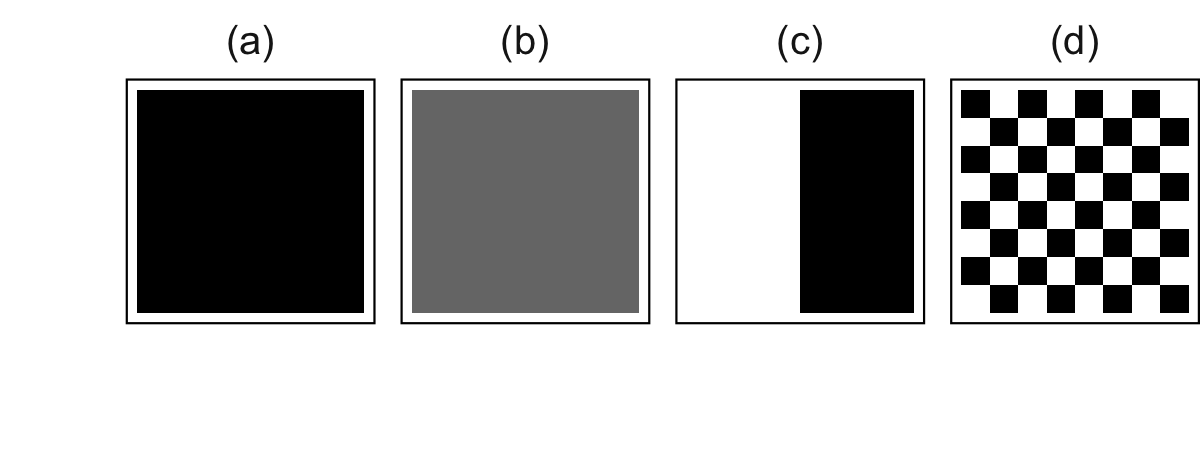
\includegraphics[width=\textwidth]{figs/checkerboard.png}
	    \end{figure}
	    \centering
	    \begin{tabular}{l c c c}
			  \textbf{City} & $H(Y)$ & $I(X,Y)$ & $J(X,Y)$ \\
			  \hline			
			  (a) & \alert{0.0} & 0.0 & 0.0\\
			  (b) & \alert{0.7} & \alert{0.0} & 0.0\\
			  (c) & 0.7 & \alert{0.7} & \alert{0.6}\\
			  (d) & 0.7 & 0.7 & \alert{2.7}\\
		\end{tabular}

	\end{frame}
	%%%%%%%%%%%%%%%%%%%%%%%%%%%%%%%%%%%%%%%%%%%%%%%%%%%%%%%%%%%%%%%%%%%%%%%%%%%%%%%%%%%%%%%%%%%
	%%%%%%%%%%%%%%%%%%%%%%%%%%%%%%%%%%%%%%%%%%%%%%%%%%%%%%%%%%%%%%%%%%%%%%%%%%%%%%%%%%%%%%%%%%%
	\begin{frame}\frametitle{A Three-Dimensional Characterization of Urban Diversity}
		\centering
		\begin{tabular}{l  c c c }%
 		    \bfseries City &  $H(Y)$  &  $I(X,Y)$  &  $J(X,Y)$ \\
 		    \hline
 	    	\csvreader[head to column names]{figs/mini_table.csv}{}% use head of csv as column names
 	    {\City & \HY & \IXY & \J \\}
    	\end{tabular}

    	\textit{Data accessed from the American Community Survey of the U.S. Census \cite{CensusRace}.
	}
	\end{frame}
	%%%%%%%%%%%%%%%%%%%%%%%%%%%%%%%%%%%%%%%%%%%%%%%%%%%%%%%%%%%%%%%%%%%%%%%%%%%%%%%%%%%%%%%%%%%
	%%%%%%%%%%%%%%%%%%%%%%%%%%%%%%%%%%%%%%%%%%%%%%%%%%%%%%%%%%%%%%%%%%%%%%%%%%%%%%%%%%%%%%%%%%%
	\begin{frame}\frametitle{Visualizing Diversity Profiles in Major Cities}
		\centering
		\begin{figure}
	    	\centering
	    	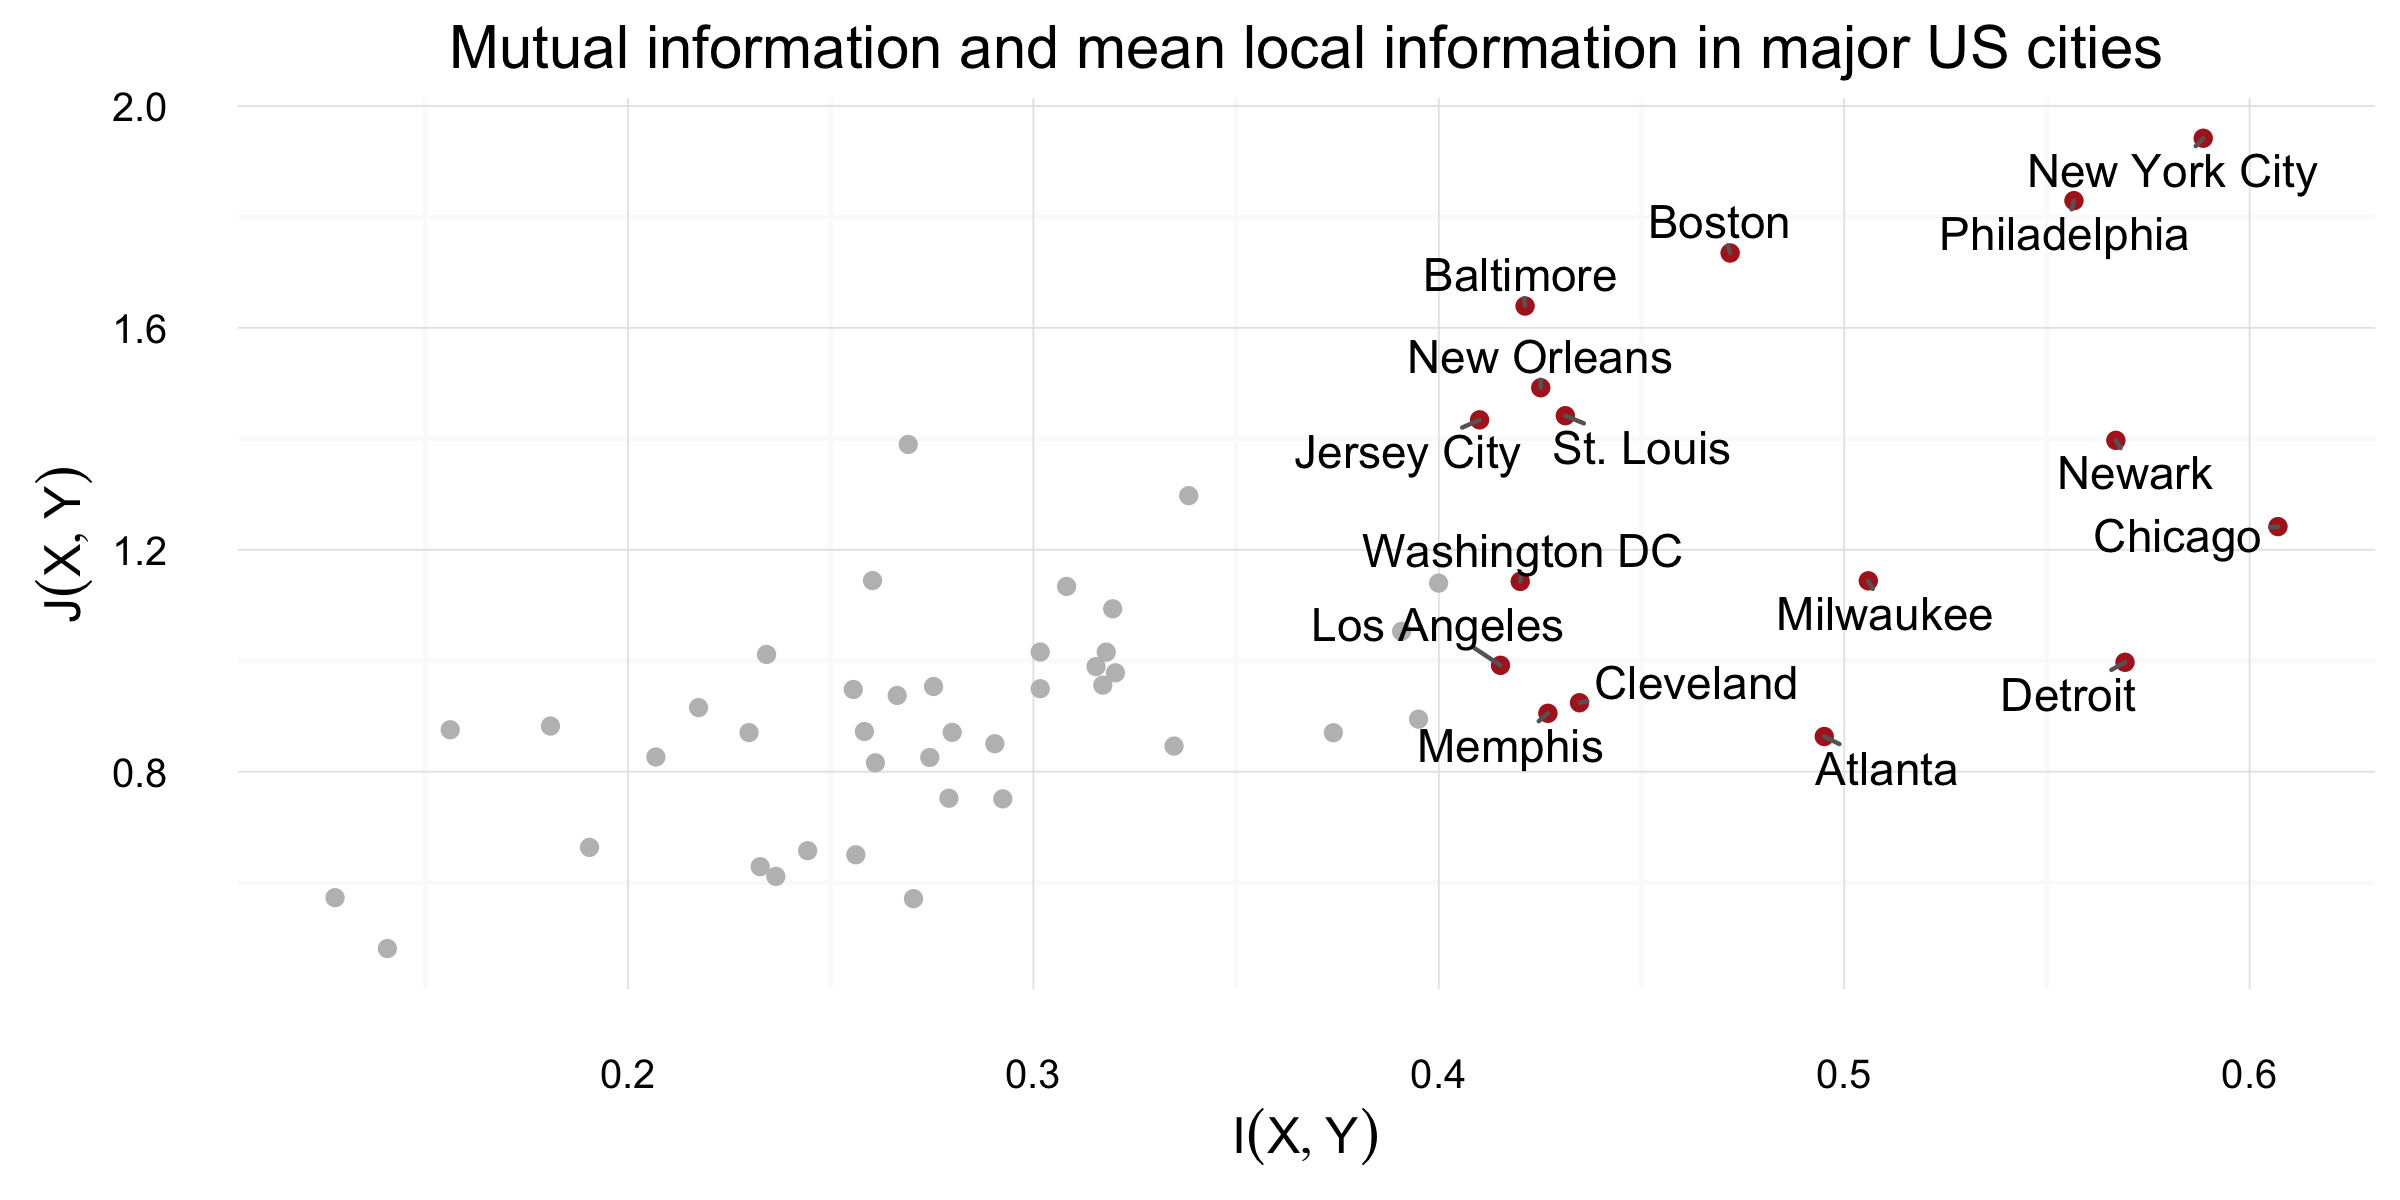
\includegraphics[width=\textwidth]{figs/mutual_fisher.png}
	    \end{figure}
	\end{frame}
	%%%%%%%%%%%%%%%%%%%%%%%%%%%%%%%%%%%%%%%%%%%%%%%%%%%%%%%%%%%%%%%%%%%%%%%%%%%%%%%%%%%%%%%%%%%
	%%%%%%%%%%%%%%%%%%%%%%%%%%%%%%%%%%%%%%%%%%%%%%%%%%%%%%%%%%%%%%%%%%%%%%%%%%%%%%%%%%%%%%%%%%%
	\begin{frame}\frametitle{Urban Density and the Compression of Social Space}
		\centering
		\begin{figure}
	    	\centering
	    	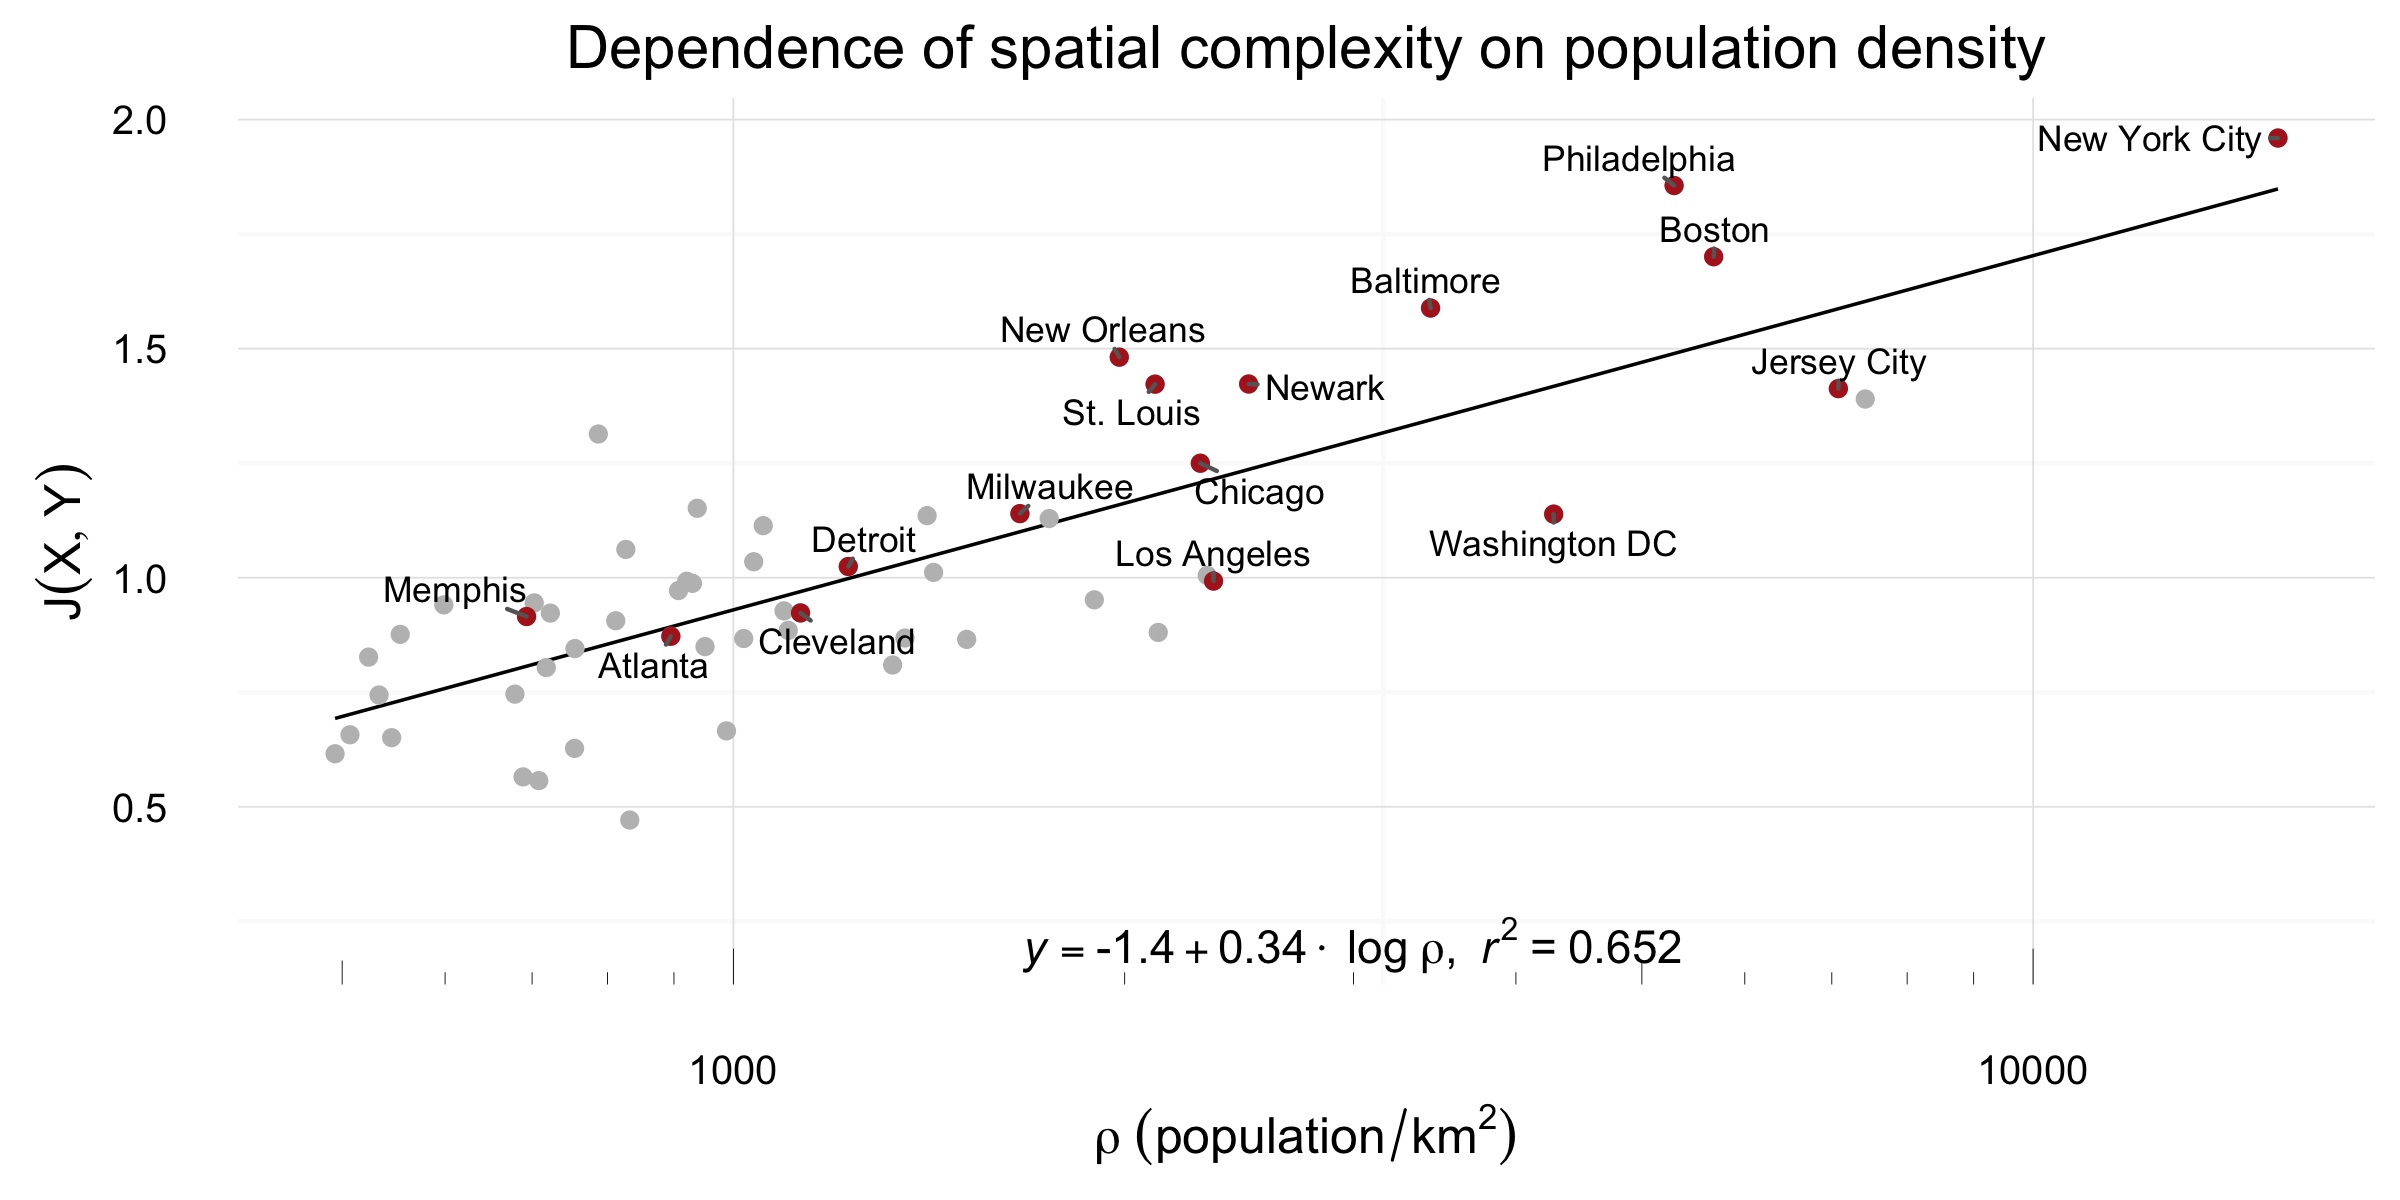
\includegraphics[width=\textwidth]{figs/density_fisher.png}
	    \end{figure}
	\end{frame}
	%%%%%%%%%%%%%%%%%%%%%%%%%%%%%%%%%%%%%%%%%%%%%%%%%%%%%%%%%%%%%%%%%%%%%%%%%%%%%%%%%%%%%%%%%%%
	%%%%%%%%%%%%%%%%%%%%%%%%%%%%%%%%%%%%%%%%%%%%%%%%%%%%%%%%%%%%%%%%%%%%%%%%%%%%%%%%%%%%%%%%%%%

	%%%%%%%%%%%%%%%%%%%%%%%%%%%%%%%%%%%%%%%%%%%%%%%%%%%%%%%%%%%%%%%%%%%%%%%%%%%%%%%%%%%%%%%%%%%
\section{Information-Theoretic Identification of Neighborhoods}
	%%%%%%%%%%%%%%%%%%%%%%%%%%%%%%%%%%%%%%%%%%%%%%%%%%%%%%%%%%%%%%%%%%%%%%%%%%%%%%%%%%%%%%%%%%%
	\begin{frame}\frametitle{How can we use this?}
		$H(Y)$, $I(X,Y)$, and $J(X,Y)$ measure diversity, evenness, and spatial exposure. 

		$J(X,Y)$ also measures ``neighborhoodiness.''
		
		\onslide<2->{Does can we use these measures to \textbf{find} neighborhoods?}

		\onslide<3->{Yes! 
			\begin{itemize}
				\item We can use $I(X,Y)$ to find neighborhoods
				\item We can use $I(X,Y)$ and $J(X,Y)$ to estimate how many we need to preserve key patterns. 
				\item So, we can view $H(Y)$, $I(X,Y)$, and $J(X,Y)$ as measurements of \textbf{complexity} in spatiosocial structure. 
			\end{itemize} 
		}

	\end{frame}

	%%%%%%%%%%%%%%%%%%%%%%%%%%%%%%%%%%%%%%%%%%%%%%%%%%%%%%%%%%%%%%%%%%%%%%%%%%%%%%%%%%%%%%%%%%%
	%%%%%%%%%%%%%%%%%%%%%%%%%%%%%%%%%%%%%%%%%%%%%%%%%%%%%%%%%%%%%%%%%%%%%%%%%%%%%%%%%%%%%%%%%%%
	\begin{frame}[t]\frametitle{Key Property of Mutual Information}
	    Suppose we cluster the locations $X$ into groups with labels $C$. 
	    \begin{block}{\only<1-2>{``Additive Organizational Decomposability'' (Chain Rule)} \only<3->{Recipe for Neighborhood Identification} }
		    \begin{equation*}
		    	\only<1-2>{I(X,Y) = \onslide<1-2>{I(C,Y)} + \onslide<1-2>{I(X,Y|C)}\;.}
		    	\only<3->{I(X,Y) = \underbrace{I(C,Y)}_\text{maximize this} + \overbrace{I(X,Y|C)}^\text{minimize this}\;.}
		    \end{equation*}
	    \end{block}
	
	    \nocite{Reardon2004} 
	    
	    \only<2>{We can use this to identify neighborhoods!} 
	    \only<4>{This optimization is hard to do exactly, but we can use a greedy approach based on hierarchical clustering.}
	\end{frame}
	%%%%%%%%%%%%%%%%%%%%%%%%%%%%%%%%%%%%%%%%%%%%%%%%%%%%%%%%%%%%%%%%%%%%%%%%%%%%%%%%%%%%%%%%%%%
	%%%%%%%%%%%%%%%%%%%%%%%%%%%%%%%%%%%%%%%%%%%%%%%%%%%%%%%%%%%%%%%%%%%%%%%%%%%%%%%%%%%%%%%%%%%
	\begin{frame}[t]\frametitle{Neighborhoods in Detroit}
	    \begin{figure}
	    	\centering
	    	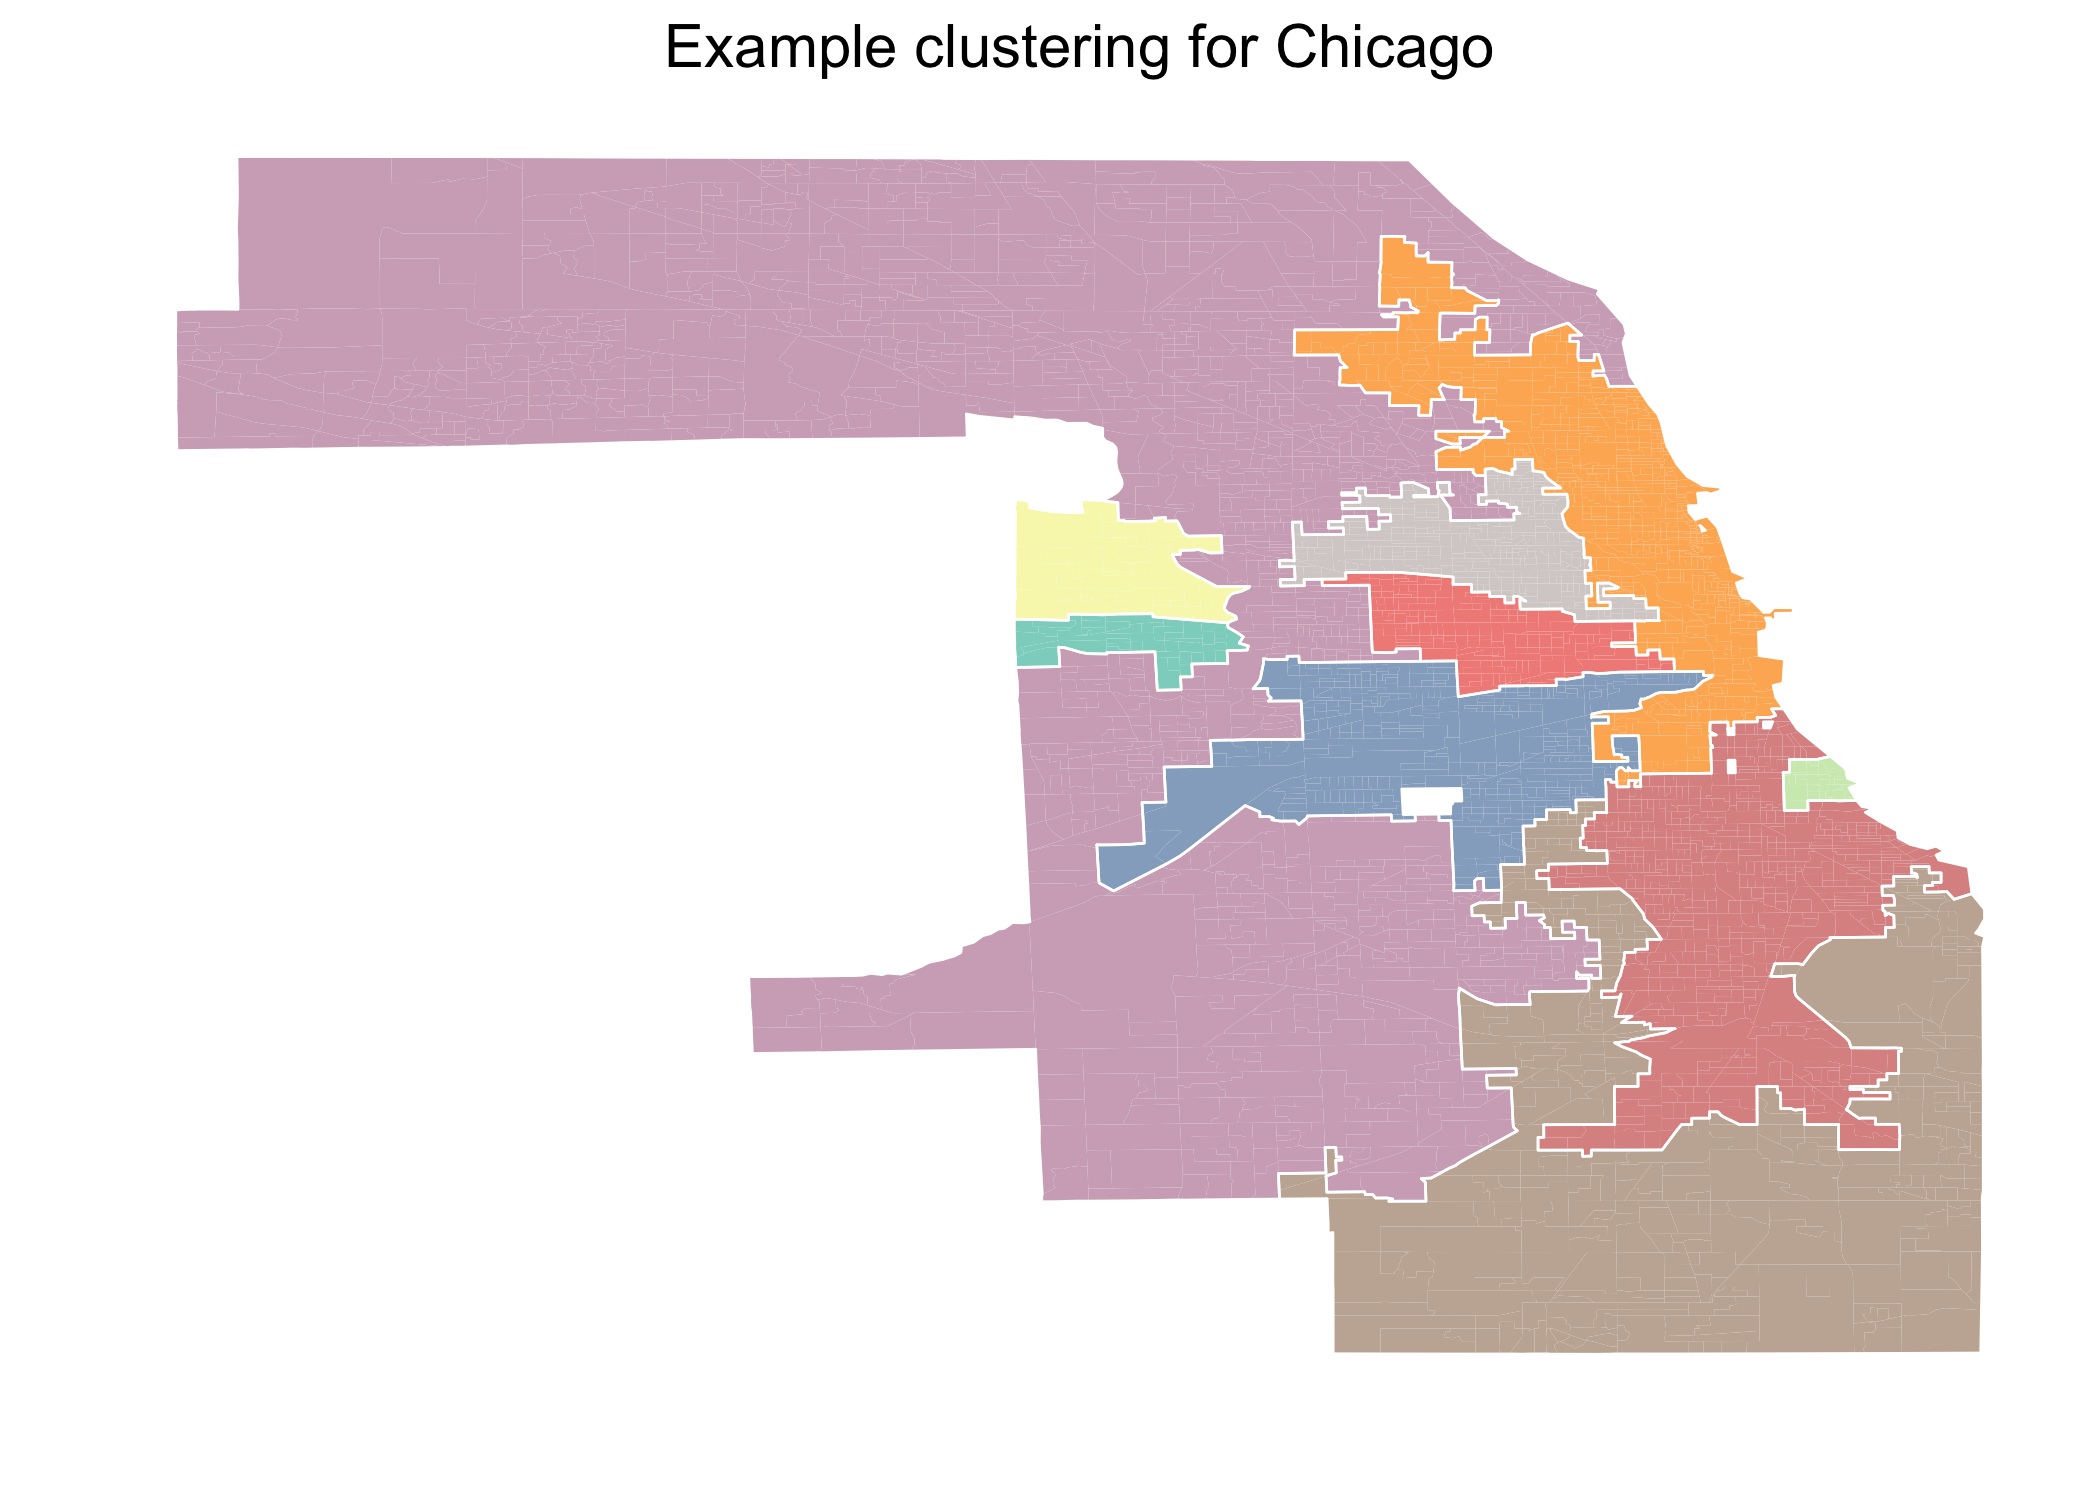
\includegraphics[width=.8\textwidth]{figs/example_cluster_map.png}

	    	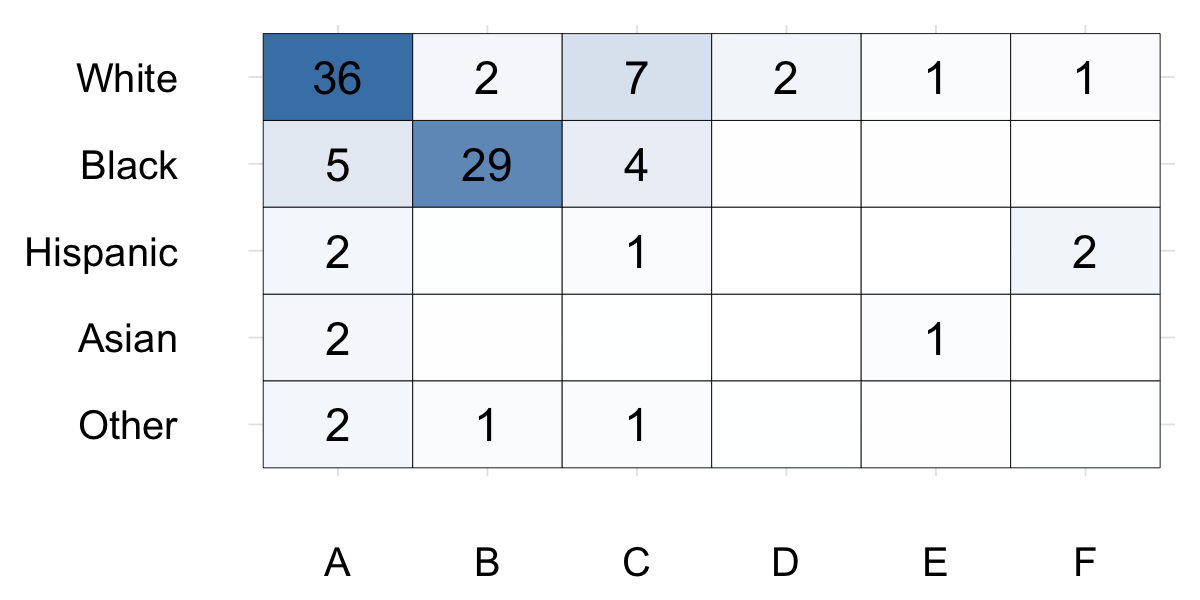
\includegraphics[width=.6\textwidth]{figs/example_clusters_detailed.png}
	    \end{figure}
	\end{frame}
	%%%%%%%%%%%%%%%%%%%%%%%%%%%%%%%%%%%%%%%%%%%%%%%%%%%%%%%%%%%%%%%%%%%%%%%%%%%%%%%%%%%%%%%%%%%
	%%%%%%%%%%%%%%%%%%%%%%%%%%%%%%%%%%%%%%%%%%%%%%%%%%%%%%%%%%%%%%%%%%%%%%%%%%%%%%%%%%%%%%%%%%%
	\begin{frame}[t]\frametitle{Information Measures and ``Clusterability''}
	    We would expect that cities with low spatial exposure $J(X,Y)$ are ``easy'' to cluster. Evaluate using ``Area Under the Curve'':

	    \begin{figure}
	    	\centering
	    	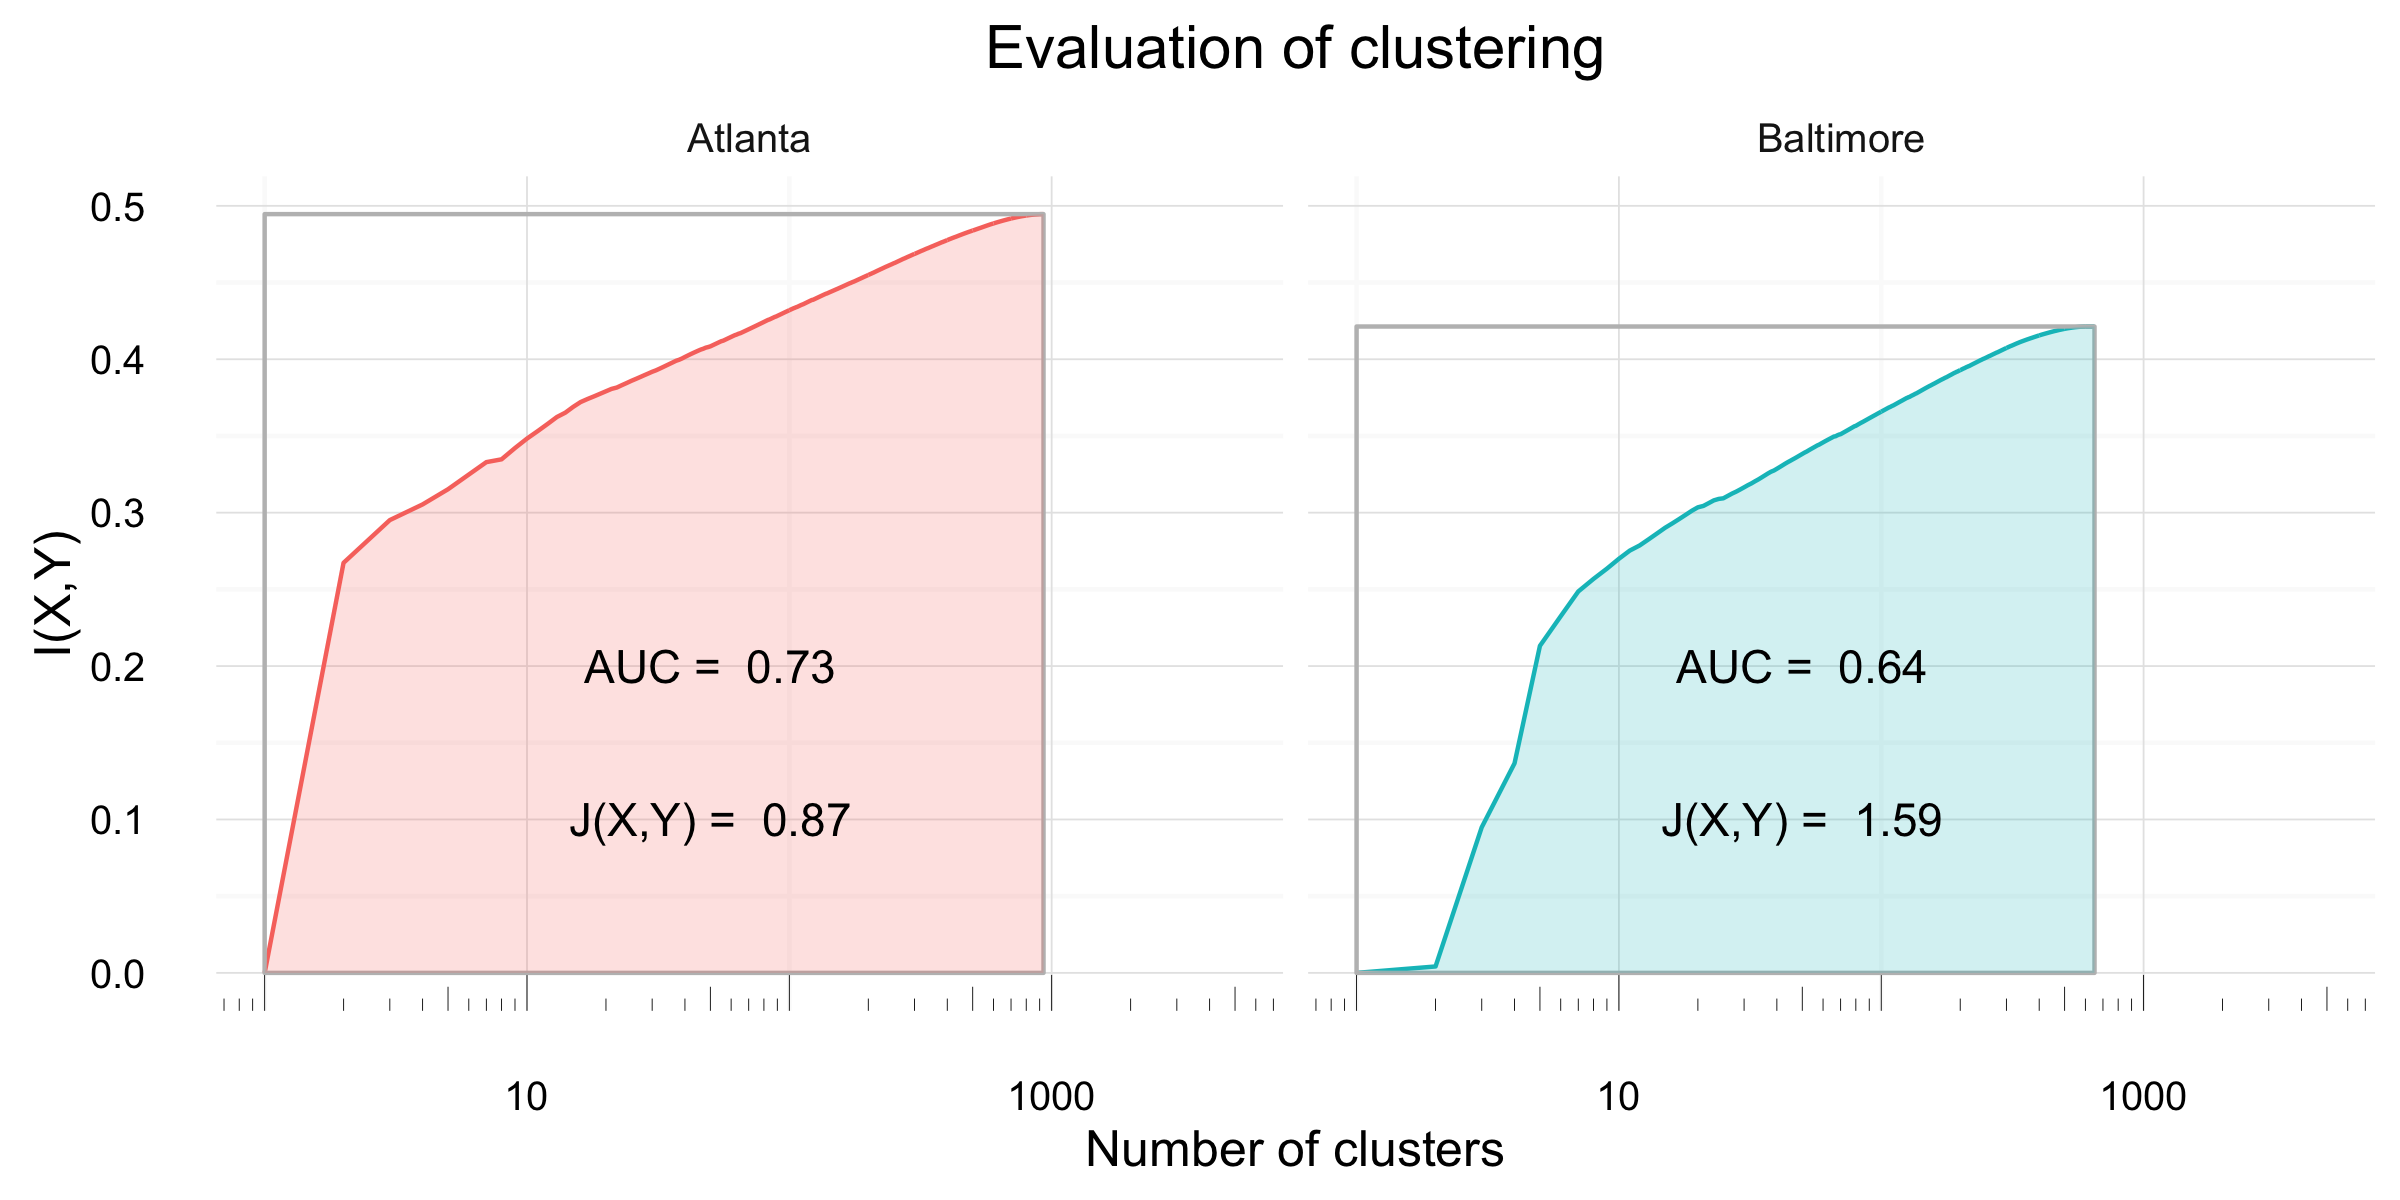
\includegraphics[width=.8\textwidth]{figs/AUC_illustration.png}
	    \end{figure}
	    Together, $H(Y)$, $I(X,Y)$ and $J(X,Y)$ explain 75\% of the variability in the clusterability (AUC) of cities. 
	\end{frame}
	%%%%%%%%%%%%%%%%%%%%%%%%%%%%%%%%%%%%%%%%%%%%%%%%%%%%%%%%%%%%%%%%%%%%%%%%%%%%%%%%%%%%%%%%%%%
\section{Wrapping Up}
	%%%%%%%%%%%%%%%%%%%%%%%%%%%%%%%%%%%%%%%%%%%%%%%%%%%%%%%%%%%%%%%%%%%%%%%%%%%%%%%%%%%%%%%%%%%
	\begin{frame}{Learnings}
		Information theory provides a natural language for the conceptualization and measurement of sociospatial variability. 

	\end{frame}
	%%%%%%%%%%%%%%%%%%%%%%%%%%%%%%%%%%%%%%%%%%%%%%%%%%%%%%%%%%%%%%%%%%%%%%%%%%%%%%%%%%%%%%%%%%%
	%%%%%%%%%%%%%%%%%%%%%%%%%%%%%%%%%%%%%%%%%%%%%%%%%%%%%%%%%%%%%%%%%%%%%%%%%%%%%%%%%%%%%%%%%%%
	\begin{frame}{Open Directions}
		Let's learn about...
	\end{frame}
	%%%%%%%%%%%%%%%%%%%%%%%%%%%%%%%%%%%%%%%%%%%%%%%%%%%%%%%%%%%%%%%%%%%%%%%%%%%%%%%%%%%%%%%%%%%
	%%%%%%%%%%%%%%%%%%%%%%%%%%%%%%%%%%%%%%%%%%%%%%%%%%%%%%%%%%%%%%%%%%%%%%%%%%%%%%%%%%%%%%%%%%%
	\begin{frame}[standout]
		Thank you! 

		Questions? 

		Feedback? 
	\end{frame}
	%%%%%%%%%%%%%%%%%%%%%%%%%%%%%%%%%%%%%%%%%%%%%%%%%%%%%%%%%%%%%%%%%%%%%%%%%%%%%%%%%%%%%%%%%%%
	%%%%%%%%%%%%%%%%%%%%%%%%%%%%%%%%%%%%%%%%%%%%%%%%%%%%%%%%%%%%%%%%%%%%%%%%%%%%%%%%%%%%%%%%%%%

% -------------------------------------------------------------------------------------------------
% APPENDIX
% -------------------------------------------------------------------------------------------------
\appendix

	%%%%%%%%%%%%%%%%%%%%%%%%%%%%%%%%%%%%%%%%%%%%%%%%%%%%%%%%%%%%%%%%%%%%%%%%%%%%%%%%%%%%%%%%%%%
	%%%%%%%%%%%%%%%%%%%%%%%%%%%%%%%%%%%%%%%%%%%%%%%%%%%%%%%%%%%%%%%%%%%%%%%%%%%%%%%%%%%%%%%%%%%

	\begin{frame}[allowframebreaks]{References}
	    
	    \bibliographystyle{plain}
	    \bibliography{/Users/phil/bibs/library.bib}
	    
	\end{frame}

	%%%%%%%%%%%%%%%%%%%%%%%%%%%%%%%%%%%%%%%%%%%%%%%%%%%%%%%%%%%%%%%%%%%%%%%%%%%%%%%%%%%%%%%%%%%
	%%%%%%%%%%%%%%%%%%%%%%%%%%%%%%%%%%%%%%%%%%%%%%%%%%%%%%%%%%%%%%%%%%%%%%%%%%%%%%%%%%%%%%%%%%%
	\begin{frame}{Relation of local and Fisher informations}
		Suppose that $p(y|x) > 0$ and that $p(y|x)$ is differentiable as a function of $x$ for all $x,y \in \mathbb{R}^n \times \mathcal{Y}$. Define $B_r \triangleq B_r(x_0) \triangleq \{ x \in \mathbb{R}^n \;|\; \lvert{x - x_0}\rvert \leq r \}$. Additionally, define the \emph{local mutual information} in $B_r$ as the mutual information between $X$ and $Y$ where $X$ is restricted to $B_r$:
		\begin{align}
			I_r(x_0) &\triangleq \mathbb{E}_X[D[p(\cdot|X)\| p(\cdot|X \in B_r)]|X \in B_r] \\
			&= \int_{B_r} p(x|X \in B_r) D[p(\cdot|x)\| p(\cdot|X \in B_r)] d^n x\;.
		\end{align}
		where $D[p\|q] \triangleq \sum_{y} p(y) \log \frac{p(y)}{q(y)}$ is the Kullback-Leibler divergence of $q$ from $p$. 
	\end{frame}
	%%%%%%%%%%%%%%%%%%%%%%%%%%%%%%%%%%%%%%%%%%%%%%%%%%%%%%%%%%%%%%%%%%%%%%%%%%%%%%%%%%%%%%%%%%%
	%%%%%%%%%%%%%%%%%%%%%%%%%%%%%%%%%%%%%%%%%%%%%%%%%%%%%%%%%%%%%%%%%%%%%%%%%%%%%%%%%%%%%%%%%%%
	\begin{frame}{Relation of local and Fisher informations}
		\begin{block}{Theorem}
		Under the stated conditions, 
			\begin{equation}
				\lim_{r\rightarrow 0} \frac{I_r(x_0)}{r^2} = \frac{n}{2(n+2)} \text{trace}\; J_Y(x_0)\;.
			\end{equation}
		\end{block}
			The Fisher information matrix $J_Y$ is given by 
			\begin{align}
				J_Y(x) &\triangleq \mathbb{E}_Y\left[\nabla_x S_{Y}(x)\nabla_x S_{Y}(x)^T \right] \\
				S_y(x) &\triangleq \log p(y|x)\;.
			\end{align}
	\end{frame}
	%%%%%%%%%%%%%%%%%%%%%%%%%%%%%%%%%%%%%%%%%%%%%%%%%%%%%%%%%%%%%%%%%%%%%%%%%%%%%%%%%%%%%%%%%%%
	%%%%%%%%%%%%%%%%%%%%%%%%%%%%%%%%%%%%%%%%%%%%%%%%%%%%%%%%%%%%%%%%%%%%%%%%%%%%%%%%%%%%%%%%%%%
	\begin{frame}\frametitle{Information Measures Check the Boxes}
		
		\begin{tabular}{l | c | c | c}
			\textbf{Criterion} & $H(Y)$ & $I(X,Y)$ & $J(X,Y)$ \\
			\hline
			Organizational Equivalence & \textcolor{mLightGreen}{\CheckmarkBold} & \textcolor{mLightGreen}{\CheckmarkBold} & \textcolor{mLightGreen}{\CheckmarkBold} \\ 
			Size/Density Invariance & \textcolor{mLightGreen}{\CheckmarkBold} & \textcolor{mLightGreen}{\CheckmarkBold} & \textcolor{mLightGreen}{\CheckmarkBold} \\ 
			Additive Group Decomposability & \textcolor{mLightGreen}{\CheckmarkBold} & \textcolor{mLightGreen}{\CheckmarkBold} & \textcolor{mLightGreen}{\CheckmarkBold} \\ 
			Additive Spatial Decomposability & NA & \textcolor{mLightGreen}{\CheckmarkBold} &  * \\
			Scale Interpretability & NA & \textcolor{mLightGreen}{\CheckmarkBold} & \textcolor{mLightGreen}{\CheckmarkBold}\\ 
			Boundary Independence & NA & \textcolor{mLightBrown}{\CheckmarkBold} & \textcolor{mLightBrown}{\CheckmarkBold} \\ 
			Exchanges & NA & \textcolor{mLightGreen}{\CheckmarkBold} & \textcolor{mLightGreen}{\CheckmarkBold}
		\end{tabular}

		* In the full paper, we argue that \cite{Reardon2004}'s version is not a workable criterion for spatial measures. 

		\textcolor{mLightBrown}{\CheckmarkBold} In the theoretical definition; in practice we are reliant on the data as it is provided. 

	\end{frame}
	%%%%%%%%%%%%%%%%%%%%%%%%%%%%%%%%%%%%%%%%%%%%%%%%%%%%%%%%%%%%%%%%%%%%%%%%%%%%%%%%%%%%%%%%%%%
	%%%%%%%%%%%%%%%%%%%%%%%%%%%%%%%%%%%%%%%%%%%%%%%%%%%%%%%%%%%%%%%%%%%%%%%%%%%%%%%%%%%%%%%%%%%
	\begin{frame}[t]\frametitle{Some Comparative Clusters of Equal Information}
	    \begin{figure}
	    	\centering
	    	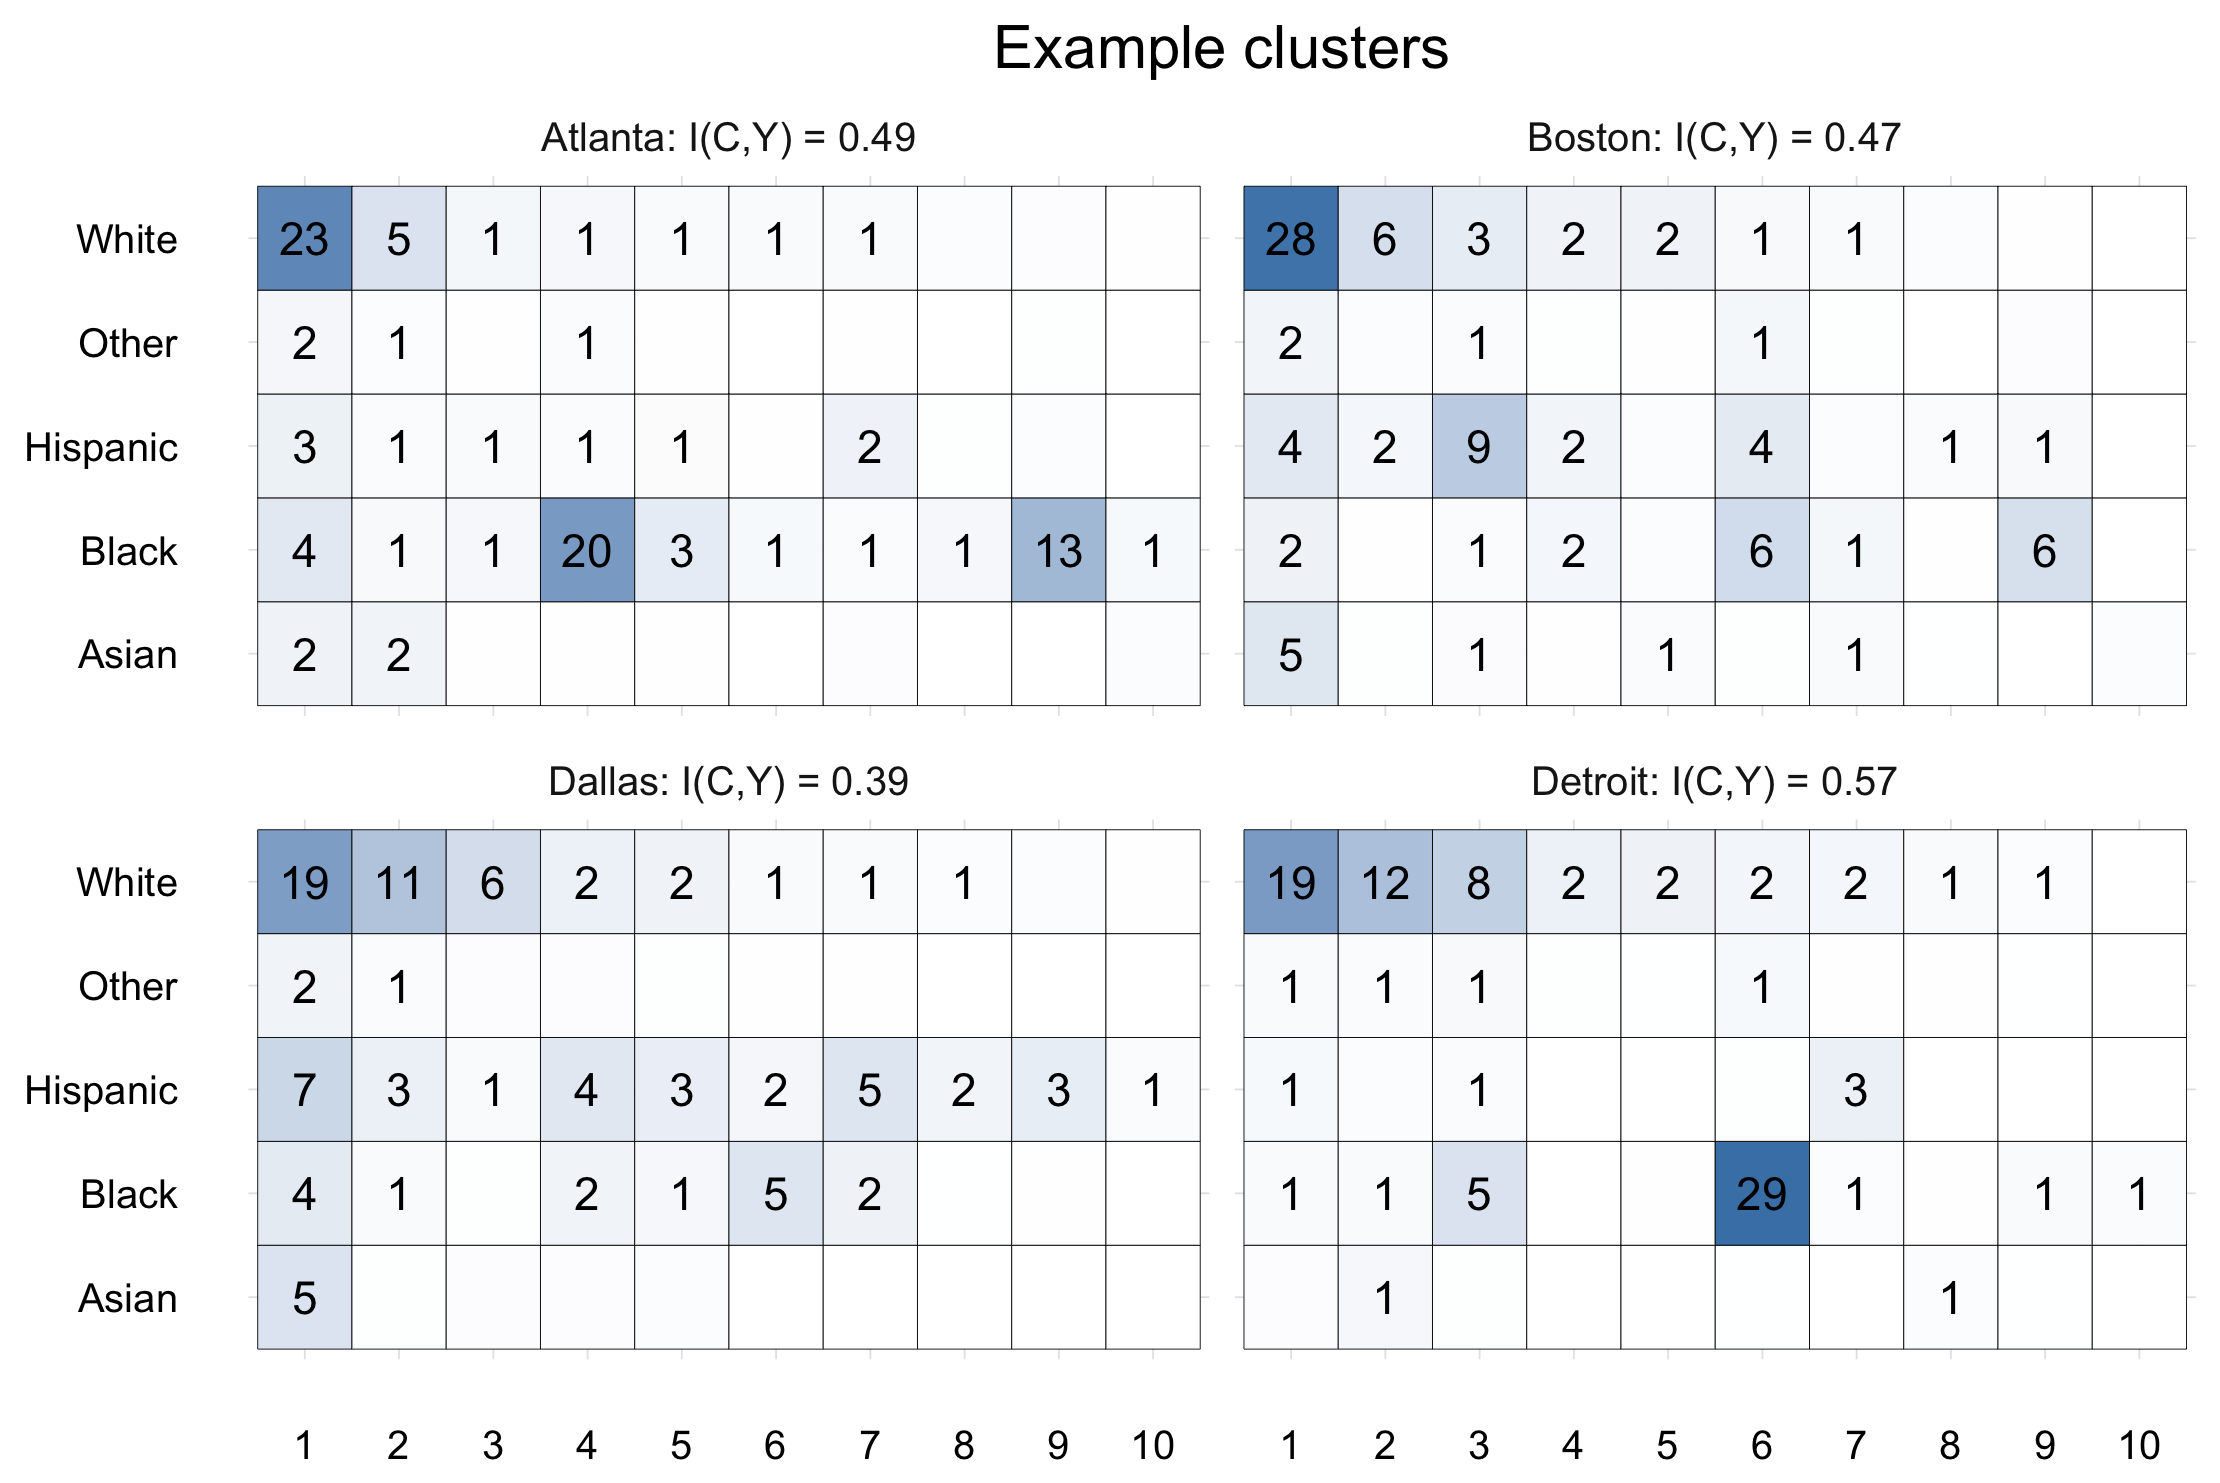
\includegraphics[width=\textwidth]{figs/example_clusters.png}
	    \end{figure}
	\end{frame}
	%%%%%%%%%%%%%%%%%%%%%%%%%%%%%%%%%%%%%%%%%%%%%%%%%%%%%%%%%%%%%%%%%%%%%%%%%%%%%%%%%%%%%%%%%%%

\end{document}